\section{辐射}\label{sec:2-7}

放在火炉旁边的物体会被烤热。热是怎样从火炉传到物体的呢?
当然不是由于对流,因为被火炉烤热的空气是上升的。
空气是热的不良导体,传导在这里也不起作用。
如果在火炉和物体之间放一块木板,木板会被烤热,而物体就不会被烤热了。
这表明,热是沿直线从火炉传给物体的。

热由物体沿直线向外射出去,叫做\textbf{辐射}。

跟传导和对流不同,用辐射方式传递热,不需要任何媒介物,可以在真空中进行。
地球上得到的太阳的热,就是通过辐射的方式传来的。

我们的地球每天都吸收太阳辐射来的大量的热。
但是,不同颜色的物体吸收太阳辐射的本领很不相同,下面我们做一个实验来研究这个问题。

\begin{figure}[htbp]
    \centering
    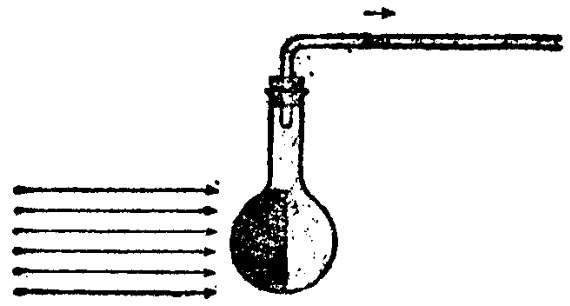
\includegraphics[width=0.5\textwidth]{../pic/czwl2-ch2-19}
    \caption{}\label{fig:2-19}
\end{figure}

利用观察气体热膨胀的实验装置,把烧瓶的一侧涂成黑色,另一侧涂成白色(图 \ref{fig:2-19})。
当太阳光照射黑色一侧时,玻璃管里的小水柱向右移动的距离大。
当太阳光照射白色一侧时,玻璃管里的小水柱向右移动的距离小。
这是因为黑色一侧从太阳辐射中吸收的热多,使烧瓶里空气的温度升得高,体积膨胀得大。
可见,\CJKunderwave{黑色表面的物体对太阳辐射的吸收本领比白色表面的物体强}。
夏天穿浅色衣服比穿深色衣服凉快些,就是这个道理。

物体表面的颜色对吸收太阳辐射有影响这一点,人们常常加以利用。
例如,飞机的表面涂成银白色,可以避免被太阳晒得过热。
相反地,人造地球卫星上的某些部件要利用太阳辐射来加热,就把这些部件涂成黑色。


